% one-figure manuscript written by fig_qc.py --tek-sekil-tex (trap T29)
\begin{figure*}[!t]
\centering
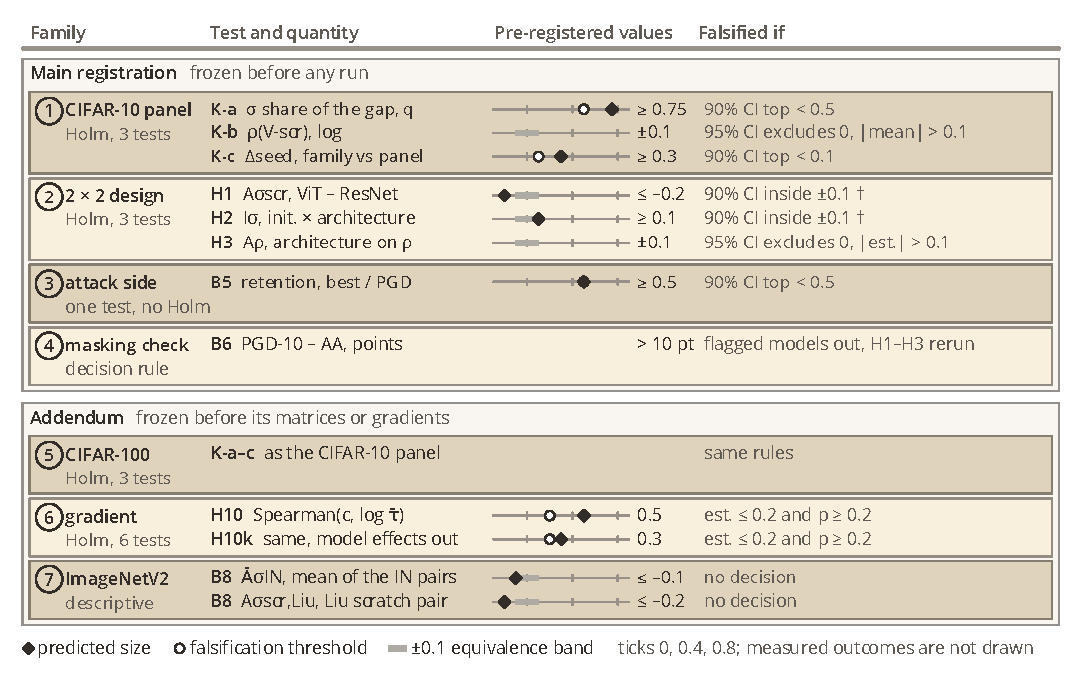
\includegraphics{fig5_registry_map}
\caption{\textbf{Registered tests and decision rules as a staircase.} Each step is one family, numbered in registration order and set behind the previous one; rows give test and quantity, place the predicted size (diamond) and falsification threshold (circle) on a number line with the ±0.1 band, and state the falsifying rule. Holm correction is per family; ImageNetV2 rows are descriptive.}
\label{fig:fig5_registry_map}
\end{figure*}
